%
% PARECE QUE ESTA LISTA, REVISAR
%

La proporci\'on de unidades no defectuosas en un proceso de fabricaci\'on es una variable aleatoria que se encuentra aproximada por
una distribuci\'on beta con una media 0.6 y una moda de 0.7, donde sus par\'ametros son $ \alpha > 1$ y $\beta > 1$
% Beta
% Media = 0.6
% Moda = 0.7
\begin{itemize}
	\item Calcule $\alpha$,$\beta$  y la varianza.\\
		% Nuevamente un sistema de ecuaciones recordando E(x) = a/(a+b) y V(x) = ab/((a+b+1)(a+b)^2)
		% Pero hay una formula para la moda , que es Moda = (a-1)/(a+b-2)
		% Con la moda y la media mesclada sacamos a y b, que son alpha y beta
		$\alpha\ =\ 0.44$\\
		$\beta\ =\ 0.76$\\
		$Varianza\ =\ V(x)\ =\ \frac{\alpha \beta}{(\alpha\ +\ \beta\ +\ 1)(\alpha\ +\ \beta)^2}\ =\ 0.105$\\
	\item ?`Cu\'al es la probabilidad de que la proporci\'on de unidades no defectuosas sea mayor que 0.5?\\
		% Como en la formula que enseno milciades es dbeta(x,a,b) donde x es la probabilidad y aca nos preguntan por la probabilidad,
		% ocupe qbeta(y,a,b) que si mal no recuerdo las "q" son la wea inversa...qbeta(0.5,0.44,0.76) y como siempre estas cuestiones
		% representan X<algo en este caso seria 1 - qbeta(0.5,0.44,0.76)
		$P(X>0.5)\ =\ 1\ -\ P(X<0.5)\ =\ 1\ -\ 0.2805213\ =\ 0.7194787$\\
	\item ?`Cu\'al es la probabilidad de que la proporci\'on de unidades no defectuosas sea igual a 0.8?\\
		Es cero! porque estamos en las continuas! aca s\'olo son rangos!\\
	\item Realice gr\'aficos de la funci\'on de densidad de probabilidad y de la funci\'on de distribuci\'on.\\
		% x<-seq(0,30,0.001) ; de ejemplo
		% plot(x,dbeta(x,0.44,0.76),type="l") % densidad
		% plot(x,pbeta(x,0.44,0.76),type="l") % distribucion
	Funci\'on de distribuci\'on:\\
  	  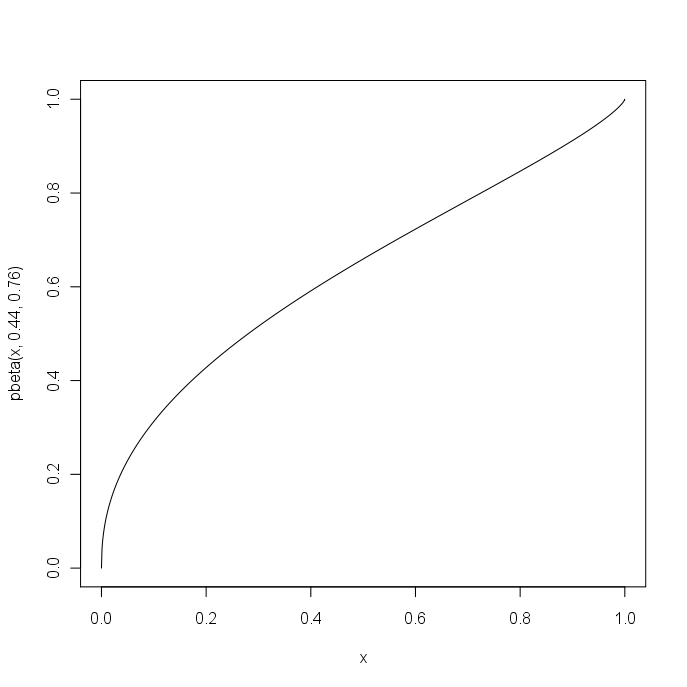
\includegraphics[width=3.3in,height=3.3in]{images/2_4-pbeta.png}\\
	Funci\'on de densidad de probabilidad:\\
  	  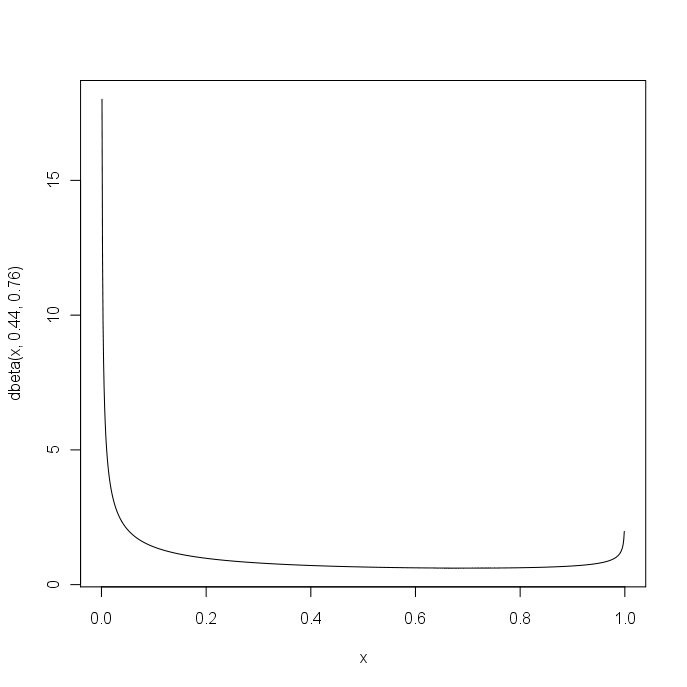
\includegraphics[width=3.3in,height=3.3in]{images/2_4-dbeta.png}

	\item Var\'ie el o los valores de los par\'ametros de la distribuci\'on y comente lo observado en los gr\'aficos de la funci\'on
	 de densidad y de distribuci\'on. (mostrando los otros perfiles de la distribuci\'on).\\\\
	Funiones de densidad:\\
	Variando el $\alpha$ a 0.5 y el $\beta$ a 0.5.\\
		% plot(x,dbeta(x,0.5,0.5),type="l",col="red") % densidad
  	  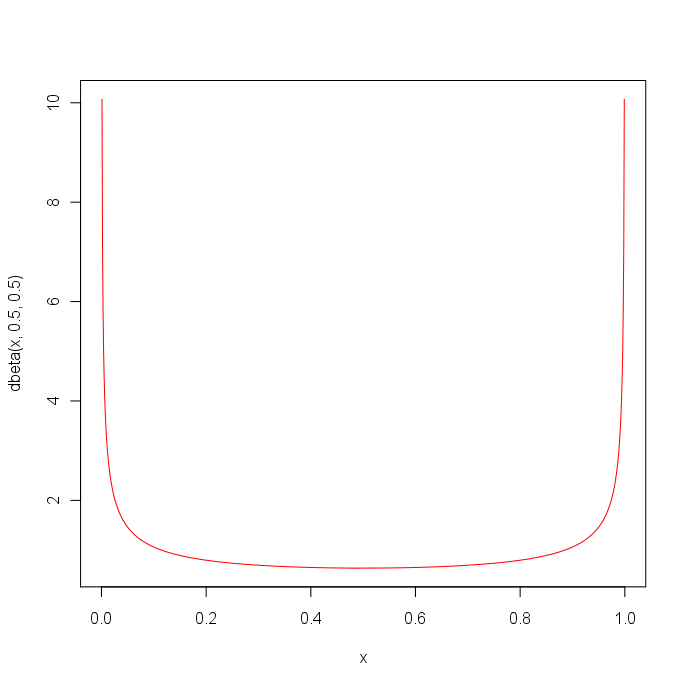
\includegraphics[width=3.3in,height=3.3in]{images/2_4-dbeta55.png}\\
	Variando el $\alpha$ a 5 y el $\beta$ a 1.\\
		% plot(x,dbeta(x,5,1),type="l",col="green") % densidad
  	  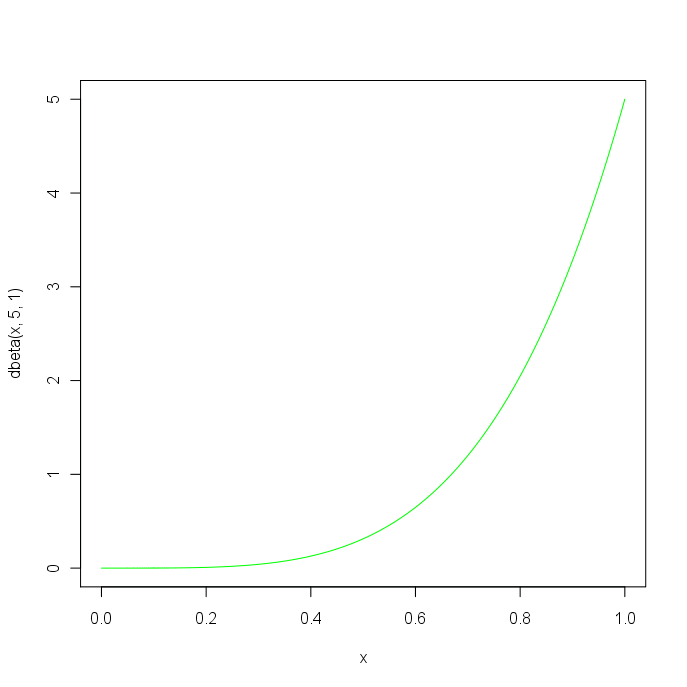
\includegraphics[width=3.3in,height=3.3in]{images/2_4-dbeta51.png}\\
	Variando el $\alpha$ a 1 y el $\beta$ a 3.\\
		% plot(x,dbeta(x,1,3),type="l",col="blue") % densidad
  	  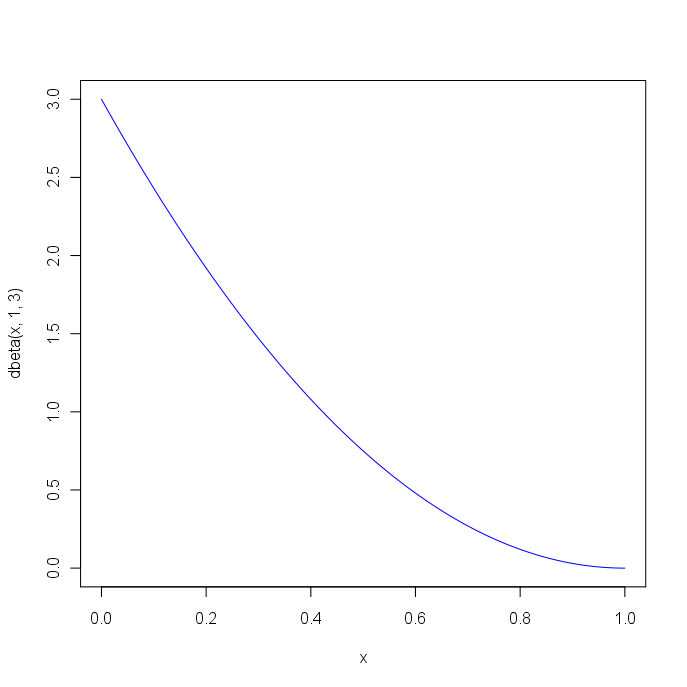
\includegraphics[width=3.3in,height=3.3in]{images/2_4-dbeta13.png}\\
	Variando el $\alpha$ a 2 y el $\beta$ a 2.\\
		% plot(x,dbeta(x,2,2),type="l",col="pink") % densidad
  	  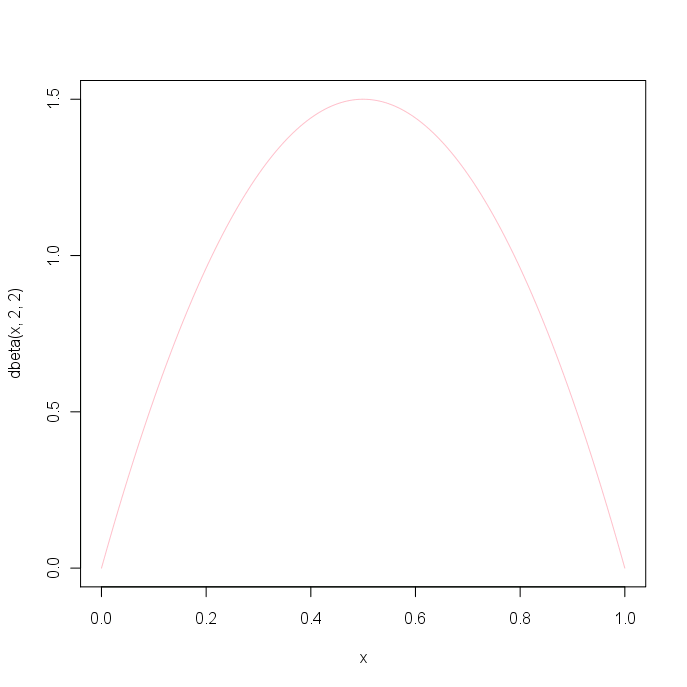
\includegraphics[width=3.3in,height=3.3in]{images/2_4-dbeta22.png}\\
	Variando el $\alpha$ a 2 y el $\beta$ a 5.\\
		% plot(x,dbeta(x,2,5),type="l",col="black") % densidad
  	  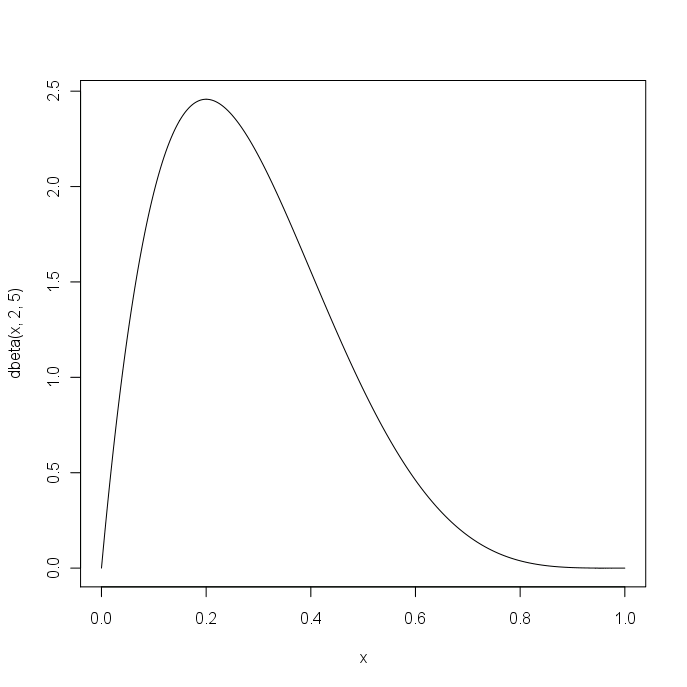
\includegraphics[width=3.3in,height=3.3in]{images/2_4-dbeta25.png}\\

	Funci\'on de distribuci\'on: Variando el $\alpha$ y el $\beta$:\\
  	  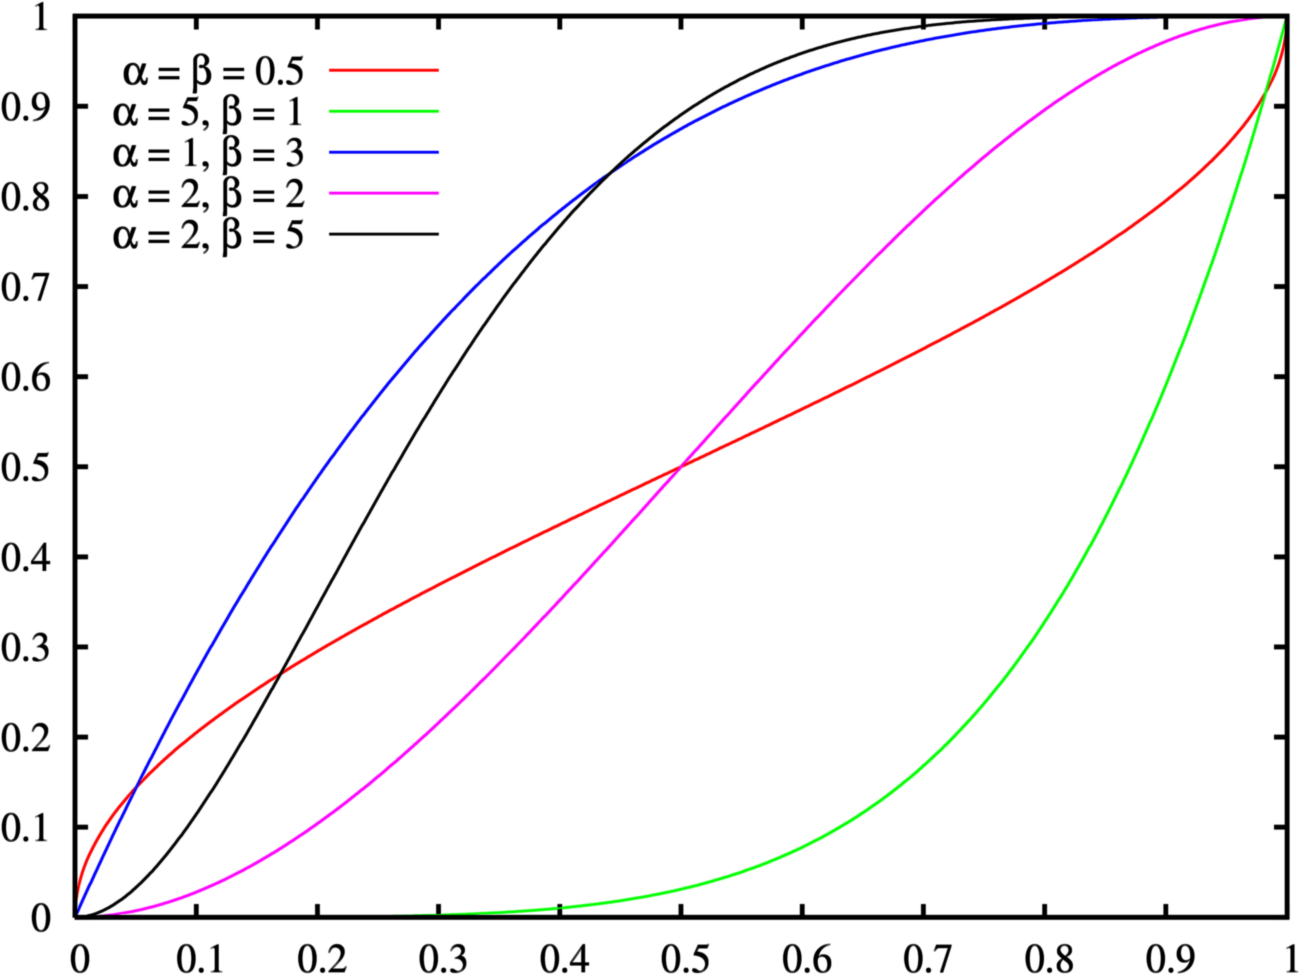
\includegraphics[height=3.3in]{images/distribucion_pbeta.png}\\
	Aca cuesta un poco mas vislumbrar la relacion. Despues de analizar los gr\'aficos, vimos que la relaci\'on entre el $\alpha$ y $\beta$ es tal que al aumentar el $\alpha$, el gr\'afico se corre hacia la izquierda en la funci\'on de densidad y en la funci\'on de distribuci\'on, mientras mas altos, mas van reduciendo el rango de valores donde x da un numero diferente de 0.

\end{itemize}
